% !TEX root = ../main.tex

\section{Hardware}
\label{sec:hardware}

The drives of \cref{sec:pair-measurement} need a known pull resistance that can be switched to either rail for every contact. \Cref{fig:frontend-final} shows how the front end of one jack provides it. The 74HC595 shift register U6 \cite{ti2026sn74hc595} latches the drive pattern and closes the switches of the TMUX1511 U15 \cite{ti2025tmux1511} to R50 and the \qty{2.5}{\volt} rail, or those of U19 to R54 and ground. The contacts of a jack thus share one resistor per rail, so only one contact per rail can be driven at a time, which is exactly the pattern of a pair measurement. The fourth channel of each four-channel TMUX1511 connects the tip switch. Each contact reaches its ADC input through a low-pass filter of \qty{10}{\kilo\ohm} and \qty{10}{\nano\farad}. The \qty{2.5}{\volt} rail is also the reference of both ADCs, so every reading is ratiometric and a drift of the rail cancels.

\begin{figure}[tb]
  \centering
  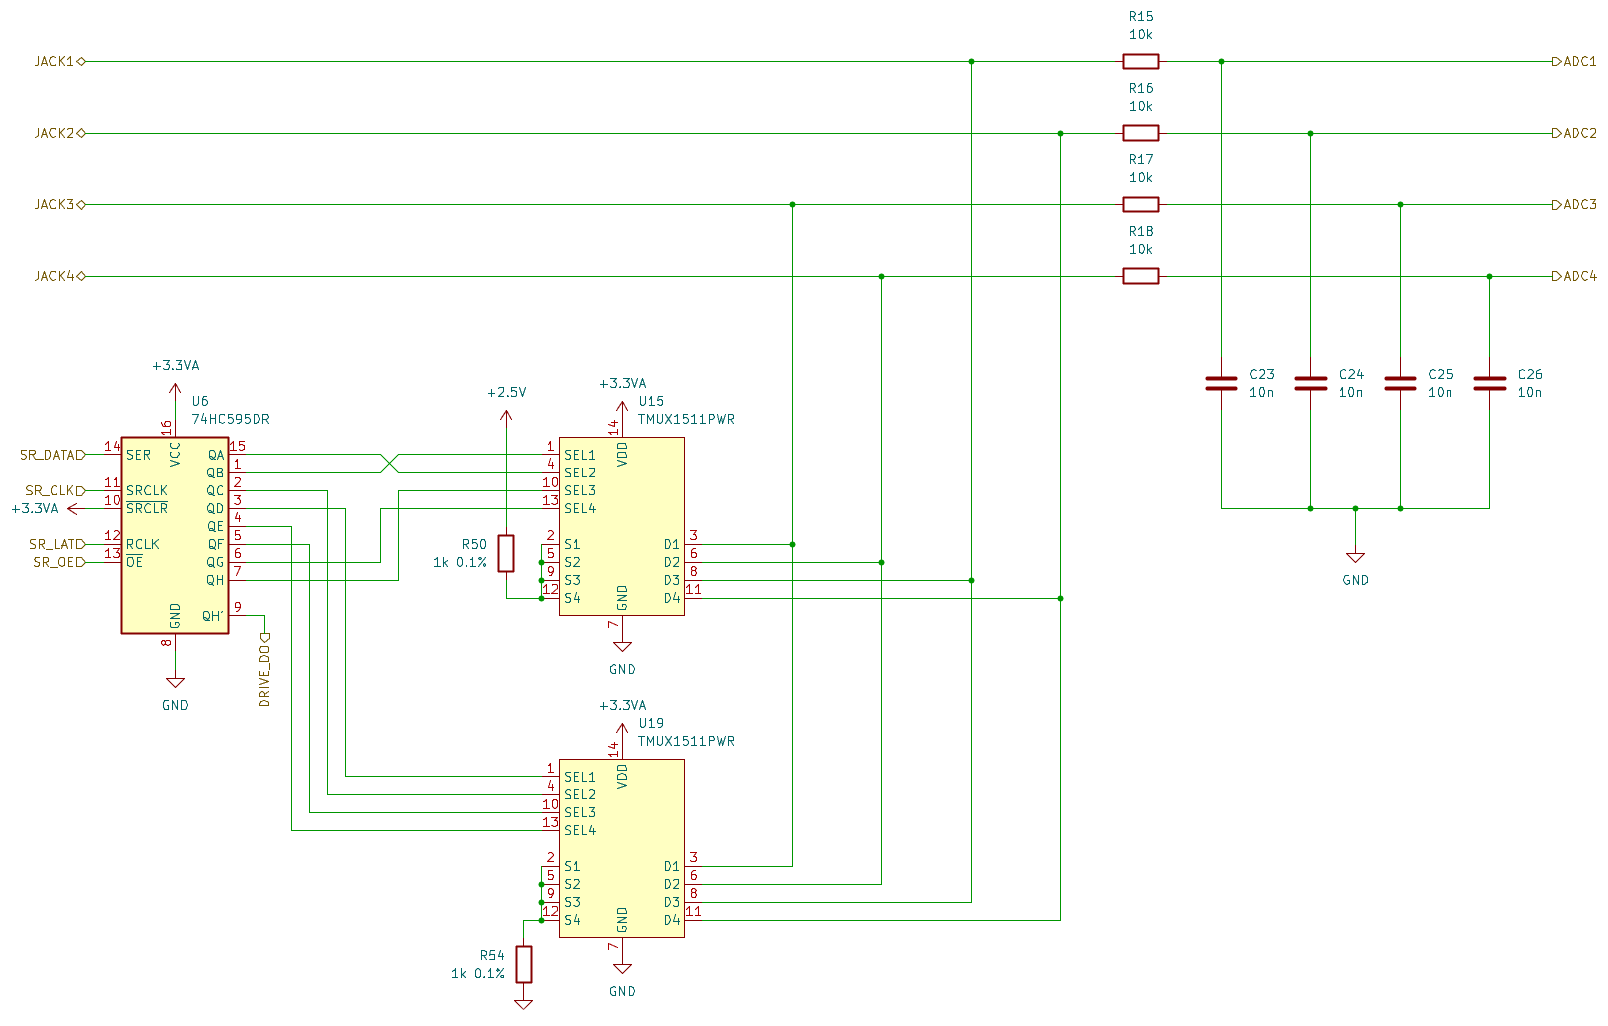
\includegraphics[width=\linewidth]{04-implementation/figures/frontend-final}
  \titledcaption{Analog Front End of One Jack}{JACK1 to JACK4 are tip, ring, sleeve and tip switch. The shift register U6 selects, per contact, a switch of U15 to the pull-up resistor R50 on the \qty{2.5}{\volt} rail or a switch of U19 to the pull-down resistor R54 on ground. R15 to R18 with C23 to C26 filter each contact before its ADC input (ADC1 to ADC4).}
  \label{fig:frontend-final}
\end{figure}

The pull resistance was chosen from the extremes of a \qty{10}{\kilo\ohm} and a \qty{500}{\kilo\ohm} pedal: with \qty{1}{\kilo\ohm}, the drop across a pull resistor is \qty{208}{\milli\volt} and \qty{5}{\milli\volt}, still ten times the noise of a reading, while the position uses a span of more than \qty{2}{\volt} in both cases (\cref{tab:pull-resistance}). When a drive changes, a floating contact charges its filter capacitor $C_\mathrm{f}$ through the pedal of total resistance $R_\mathrm{tot}$ and the filter resistor $R_\mathrm{f}$ \cite{horowitz2015art}, so the firmware waits two time constants,
\begin{equation}
  t_\mathrm{settle} = 2\,(R_\mathrm{tot} + R_\mathrm{f})\,C_\mathrm{f},
  \label{eq:settling}
\end{equation}
bounded to \qtyrange{1}{400}{\milli\second}. A \qty{100}{\kilo\ohm} pedal gives $t_\mathrm{settle} = 2 \cdot \qty{110}{\kilo\ohm} \cdot \qty{10}{\nano\farad} = \qty{2.2}{\milli\second}$, whereas for a \qty{10}{\kilo\ohm} pedal the lower bound applies. Two time constants alone leave about \qty{13.5}{\percent} of a step, but the sinc\textsuperscript{3} filter of the AD7718 then averages the input over about three conversion periods, \qty{3.7}{\milli\second} at the rate chosen in \cref{sec:firmware}, while the capacitor keeps settling \cite{adi2001ad7718}, so the remaining error is averaged down well below the noise of a reading.

Both AD7718 ADCs \cite{adi2001ad7718} run in ten-channel mode and read two jacks each. On both, AIN6 is grounded and AIN10 is tied to the \qty{2.5}{\volt} rail for a self-test of the conversion path. Every SPI and shift-register line has a \qty{47}{\ohm} series resistor at its driver, so that driver and resistor together approach the line impedance, which removes overshoot and reduces emission \cite{ti1998scaa031}. The \qty{5}{\volt} regulator also supplies the four WS2812B LEDs \cite{worldsemi2026ws2812b}, whose brightness the firmware limits to 10 of 255, about \qty{4}{\percent}, because the bare LEDs without a diffuser are already bright at that level. The schematics (\cref{fig:schematic-microcontroller,fig:schematic-analog-frontend,fig:schematic-channel-j2,fig:schematic-power,fig:schematic-leds}) became a two-layer printed circuit board (PCB), manufactured by Aisler and assembled by hand with 15 test points (\cref{fig:pcb}).

The design reached this form over the proposal \cite{benson2026proposal}, the circuit of the first milestone presentation of the course (milestone~1) and a breadboard prototype (\cref{tab:design-decisions}). Milestone~1 had replaced the analog switches of the proposal by tristate buffers. The final board returns to switches, since the current in \cref{eq:pair} needs a known pull resistance, whereas the output impedance of a buffer is specified only as a voltage-dependent range \cite{ti2026sn74lvc126a}.

\begin{table}[tb]
  \centering
  \footnotesize
  \titledcaption{Design Decisions}{Components planned in the proposal and at milestone~1 against those on the final PCB, with the reason for each change. The breadboard prototype already used the AD7718 and the SN74LVC126A buffers.}
  \label{tab:design-decisions}
  \begin{tabularx}{\linewidth}{@{}>{\raggedright\arraybackslash}p{0.12\linewidth} >{\raggedright\arraybackslash}p{0.19\linewidth} >{\raggedright\arraybackslash}p{0.19\linewidth} >{\raggedright\arraybackslash}X@{}}
    \toprule
    \textbf{Block} & \textbf{Planned} & \textbf{Final PCB} & \textbf{Reason} \\
    \midrule
    ADC & ADS8688 or ADS1241 (proposal), AD7124-8 (milestone~1) & 2$\times$ AD7718 & ADS8688 oversized (\num{500000} samples per second, \qty{+-10.24}{\volt}, \qty{5}{\volt} supply) \cite{ti2015ads8688}; ADS1241 at most 15 samples per second \cite{ti2013ads1241}; AD7124-8 only as LFCSP, unsuited to hand assembly \cite{adi2026ad7124}; AD7718: 24 bit, \qtyrange{2.7}{3.6}{\volt}, up to \qty{1365}{\hertz}, ten inputs, SOIC-28 \cite{adi2001ad7718} \\
    Pull switching & TS5A23157 switches \cite{ti2026ts5a23157} (proposal), SN74LVC126A (milestone~1) & 2$\times$ TMUX1511 per jack, \qty{1}{\kilo\ohm} \qty{0.1}{\percent} per rail & buffer output impedance only specified as a voltage-dependent range \cite{ti2026sn74lvc126a}; switch on-resistance \qty{2}{\ohm} \cite{ti2025tmux1511}; 74HC125-type buffers not available in the required package \\
    Supply, ground & separate analog supply, star point & one \qty{3.3}{\volt} rail, \qty{2.5}{\volt} pull-up rail and reference, one ground & small two-layer board; switches and ADCs join digital and analog pins, so a split ground would enlarge the board and lengthen the SPI lines \cite{kester2009mt031}; low-noise LDOs instead \cite{adi2025adp7142} \\
    Input filter & \qty{1}{\kilo\ohm}, \qty{100}{\nano\farad} & \qty{10}{\kilo\ohm}, \qty{10}{\nano\farad} & same corner (\qty{1.6}{\kilo\hertz}), a tenth of the capacitance, so faster settling; \qty{26}{\decibel} at the \qty{32.768}{\kilo\hertz} modulator rate, which the digital filter passes; buffered ADC inputs accept \qty{10}{\kilo\ohm} \cite{adi2001ad7718, andrews2015deltasigma} \\
    Input protection & LM74700 ideal-diode controller & fuse, suppressor diode, P-channel MOSFET; \qty{9}{\volt} center negative & LM74700 is an automotive battery controller \cite{ti2020lm74700}; minimal circuit for \qtyrange{9}{12}{\volt} pedal supplies and their polarity \cite{roland2026psas}; no rectifier, to avoid complexity and noise \\
    Micro\-controller & STM32G4 or RP2040 & Raspberry Pi Pico~2~W (RP2350) & tested module with USB, crystal and flash; two SPI buses, debug probe, WiFi \cite{rpi2026pico2w, rpi2026rp2350} \\
    \bottomrule
  \end{tabularx}
\end{table}
